%  !TeX  root  =  user_guide.tex

\section{R�umliche Abfrage Plugin}\label{sec:spatial_query}

% when the revision of a section has been finalized, 
% comment out the following line:
% \updatedisclaimer

Das \toolbtntwo{spatialquery}{R�umliche Abfrage} Plugin erm�glicht eine r�umliche 
Abfrage (Objekte ausw�hlen) in einem Quelllayer mit Verweis auf einen Referenzlayer. 
Die Funktionalit�t basiert auf der GEOS-Bibliothek und ist abh�ngig von dem 
ausgew�hlten Datentyp (Punkt, Linie, Polygon) des Layers mit den Quellobjekten.

M�gliche Operatoren sind:

\begin{itemize}[label=--]
\item Ber�hrt
\item Enth�lt
\item Gleicht
\item Innerhalb
\item Ist ausserhalb
\item �berlappt
\item �berschneidet
\item Kreuzt
\end{itemize}

\minisec{Verwendung der Erweiterung}

Als Beispiel sollen die Regionen Alaskas gefunden werden, die Flugpl�tze enthalten. 
Folgende Schritte sind notwendig.

\begin{enumerate}
  \item Starten Sie QGIS und laden Sie die Vektorlayer regions.shp und airports.shp. 
  \item Laden Sie das R�umliche Abfrage Plugin im Plugin Manager (Siehe Kapitel 
  \ref{sec:load_core_plugin}) und klicken Sie auf das Icon 
  \toolbtntwo{spatialquery}{R�umliche Abfrage}, das in der Werkzeugleiste erscheint. 
  Der Dialog der Erweiterung �ffnet sich, wie in Abbildung \ref{fig:spatialquerysample} 
  zu sehen.
  \item W�hlen Sie den Layer regions als Layers mit den Quellobjekten und airports als 
  Layer mit den Referenzobjekten aus.
  \item W�hlen Sie 'Enth�lt' als Operator und klicken Sie dann auf \button{Anwenden}.
\end{enumerate}

Sie bekommen dann eine Liste von Objekt IDs und haben verschiedene Optionen.

\begin{itemize}[label=--]
\item Klicken Sie auf \toolbtntwo{selectesubsetlayer}{Layer mit Liste von Elementen erzeugen}
\item W�hlen Sie eine ID aus der Liste und klicken Sie auf 
\toolbtntwo{selectcreatelayer}{Layer mit gew�hlten erzeugen}
\item W�hlen Sie \button{Aus aktueller Auswahl entfernen} im Bereich 'Das Ergebnis speichern in'.
\item Zus�tzlich k�nnen Sie die Kontrollk�stchen \checkbox{Zum Element zoomen} oder 
\checkbox{Protokoll} aktivieren.
\end{itemize}

\begin{figure}[ht]
   \centering
   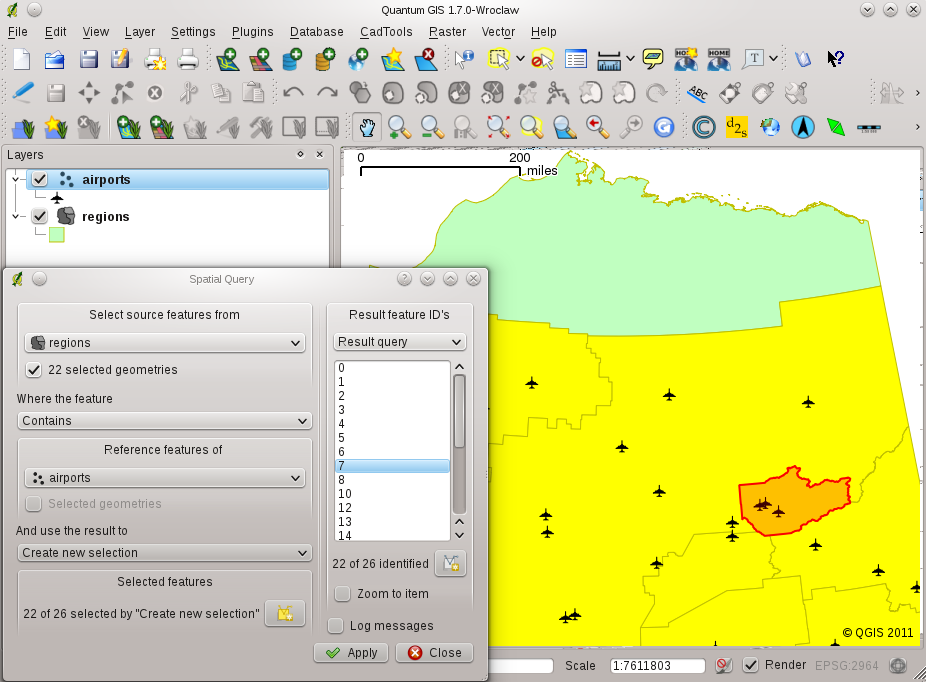
\includegraphics[clip=true, width=14cm]{spatial_query_sample}
   \caption{R�umliche Abfrage - Regionen Alaskas mit Flugpl�tzen \nixcaption}
   \label{fig:spatialquerysample}
\end{figure}

\FloatBarrier

